\begin{title}[\Large]
  Криволинейные интегралы первого рода
\end{title}

\begin{block}[Кривая]
  Кривая это упорядоченное множество точек $\Gamma \subset R^3$

  $\vec \varphi = \vec \varphi(t) = (x(t), y(t), z(t)) ~~~ t = [a,b]$

  $R \to R^3$ непрерывно

  $\vec \varphi(a)$ начальная точка кривой

  $\vec \varphi(b)$ конечная точка кривой

  $\vec \varphi([a,b]) \not= 0$ тогда гладкая

  Кривая называется кусочно гладкая если каждая гладкая часть начинается с
  другой гладкой части (может быть разорвано)

  $\vec \rho = \vec \rho(\tau) = (u(\tau), v(\tau), w(\tau)) ~~
  \tau \in [\alpha, \beta]$

  $\vec \rho$ эквивалентна $\vec \varphi$ если $\exists$ взаимооднозначное
  отображение, $\nearrow$, $t'(\tau) > 0$ тогда замена параметра допустима

  $\vec \rho(\tau) = (x(t(\tau)) = v(\tau), y(t(\tau)) = u(\tau),
  z(t(\tau)) = w(\tau))$
\end{block}

\begin{define}[криволинейным интегралом первого рода]
  $\Gamma \subset R^3$ частично гладкая кривая $\vec \varphi = \vec \varphi(t) =
  (x(t), y(t), z(t)) ~~ t \in [a,b]$ и $f(x,y,z)$ непрерывна на $\Gamma$ тогда
  криволинейным интегралом первого рода $f(x,y,z)$ называется определенный
  интеграл
  $$
  \int_a^b f(x(t), y(t), z(t))|\vec \varphi'(t)|dt =
  \int_{\Gamma} f(x,y,z) d l
  $$
\end{define}

\begin{theorem}
  Криволинейный интеграл 1-ого рода не зависит от способа задания кривой
  $\Gamma$
\end{theorem}

\begin{proof}
  $$
  \int_a^b f(x(t), y(t), z(t))|\vec \varphi'_t(t)|dt =
  \int_{\alpha}^{\beta} f(v(\tau), u(\tau), w(\tau))
  |\vec \rho'_{\tau}(\tau)|d\tau =
  $$
  $$
  = \int_{\alpha}^{\beta} f(x(t(\tau)), y(t(\tau)), z(t(\tau)))
  |\vec \varphi'_t(t(\tau))| t'(\tau)d\tau =
  $$
  $$
  = \int_{\alpha}^{\beta} f(v(\tau), u(\tau), w(\tau))
  |\vec \varphi'_t(t(\tau))| d\tau =
  $$
  $$
  = \int_{\alpha}^{\beta} f(v(\tau), u(\tau), w(\tau))
  |\vec \rho'_{\tau}(t(\tau))| d\tau =
  $$
\end{proof}

\begin{theorem}
  Криволинейный интеграл не зависит от ориентации кривой $\Gamma$
  $$
  \int_{\Gamma} f(x,y,z) d l = \int_{\Gamma^-} f(x,y,z) d l
  $$
  $\vec \rho (\tau) = \vec \varphi (a+b-\tau) ~~ \tau \in [a,b]$
  $$
  \int_{\Gamma^-} f(x,y,z) d l = \int_a^b
  f(x(a+b-\tau),y(a+b-\tau),z(a+b-\tau)) |\varphi'_{\tau}(a+b-\tau)|d \tau =
  $$
  $$
  = |a+b-\tau=t ~~ dt = -d\tau| = \int_a^b f(x(t),y(t),z(t))
  |\vec \varphi'_t(t)| dt = \int_{\Gamma} f(x,y,z) dl
  $$
\end{theorem}

\begin{theorem}
  $\Gamma$ кусочно гладкая кривая $\Gamma = \Gamma_1 \cup \Gamma_2 \cup
  \ldots \cup \Gamma_m$
  $$
  \int_{\Gamma} f(x,y,z) d l = \sum_{k=1}^m \int_{\Gamma_k} f(x,y,z) d l
  $$
\end{theorem}

\begin{title}[\Large]
  Криволинейный интеграл второго рода
\end{title}

\begin{define}[плоского поля]
  Если можно так выбрать систему координат что $Q$ или $P$ или $R$ $\equiv 0$
  тогда поле плоское.
\end{define}

\begin{define}
  $\Gamma \subset \Omega$ $\vec \varphi = \vec \varphi(t) = (x(t), y(t), z(t))$
  криволинейным интегралом второго рода называет определенный интгерал
  $$
  \int_a^b (P(x(t), y(t), z(t))x'(t) + Q (x(t), y(t), z(t))y'(t) +
  R(x(t), y(t), z(t))z'(t))dt =
  $$
  $$
  = \int_{\Gamma} (\vec F, d \vec \varphi) =
  \int_{\Gamma} Pdx + Qdy + Rdz
  $$
\end{define}

\begin{theorem}
  Криволинейный интеграл второго рода не зависит от выбора парамтризации

  $\vec \varphi = \vec \varphi(t) = (x(t), y(t), z(t))$

  $\vec \rho = \vec \rho(\tau) = (u(\tau), v(\tau), w(\tau)) ~~ \tau \in
  [\alpha, \beta]$
  $$
  \int_{\Gamma} (\vec F, d \vec \varphi) = \int_{\Gamma}(\vec F, d\vec \rho)
  $$
\end{theorem}

\begin{theorem}
  $$
  \int_{\Gamma^-} (\vec F, d\vec \varphi) = - \int_{\Gamma} (\vec F, d \vec
  \varphi)
  $$
\end{theorem}

\begin{proof}
  $\vec \varphi = \vec \varphi(t) = (x(t), y(t), z(t)) ~~ t \in [a,b]$

  $\vec \rho = \vec \rho (\tau) = \vec \varphi(a+b-\tau) ~~ \tau \in [a,b]$
  $$
  \int_{\Gamma^-}(\vec F, d\vec \phi) = \int_a^b \vec F(u(\tau), v(\tau),
  w(\tau)d\vec \rho (\tau)) =
  $$
  $$
  = \int_a^b \vec F(x(a+b-\tau),y(a+b-\tau),z(a+b-\tau))d\vec \varphi(a+b-\tau)
  =
  $$
  $$
  |a+b -\tau = t ~~ d\tau = -dt|
  = \int_a^b \vec F(x(t), y(t), z(t))d\vec \varphi(t) =
  - \int_a^b \vec F(x,y,z)d\vec\varphi
  $$
  $$
  d\vec \rho(\tau) = \vec \rho'_{\tau} d\tau = \vec \varphi'_t \rho'_{\tau}
  d\tau = -\vec \varphi'_t d\tau
  $$
\end{proof}

\begin{theorem}
  $\Gamma = \Gamma_1 \cup \Gamma_2 \cup \ldots \cup \Gamma_m$
  $$
  \int_{\Gamma^-} (\vec F, d\vec \varphi) = \sum_{k=1}^m \int_{\Gamma_k}
  (\vec F, d\vec \varphi)
  $$
\end{theorem}

\begin{define}[односвязаной области]
  $D \subset R^2$ область называется односвязной если ограниченная часть
  плоскости ограничена контуром часть плоскости $Q$ польностью содержит кривую.

  По колхозному: односвязанная область это область без дырок.
\end{define}

\begin{block}[Формула Грин]
  $D \subset R^2$ односвязанная область где $(P,Q)$ непрерывно дифференцируемое
  поле тогда $\forall \Gamma \subset D$ $\Gamma = \partial \Omega$ замкнута и
  ориентация против часовой стрелки
  $$
  \int_{\Gamma} Pdx + Qdy = \iint_{\Omega}  \left( \frac{\partial Q}{\partial x}
  - \frac{\partial P}{\partial y} \right) dxdy
  $$
\end{block}

\begin{proof}
  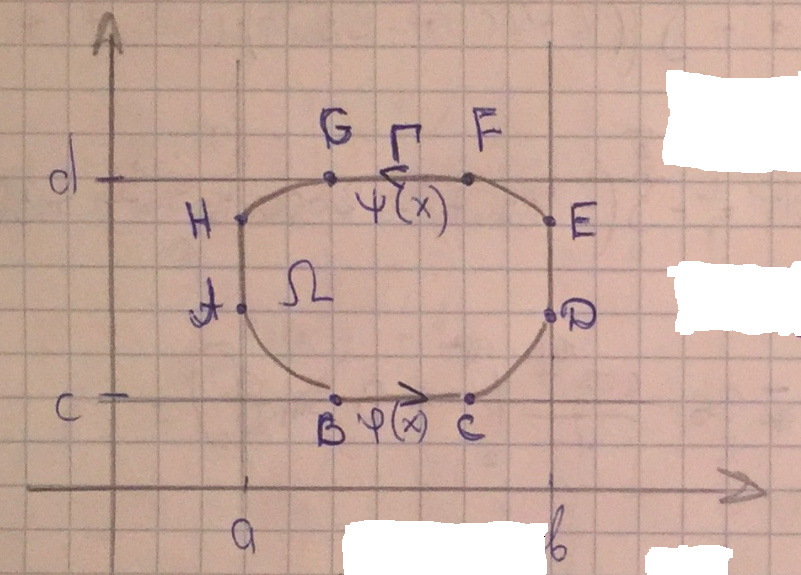
\includegraphics[width = 6cm]{formulaGrin}

  Докажем для $\Omega$ элементарный относительно обеих осей

  1)
  $\Gamma_{ABCD}: y = \varphi(x) ~~ x \in [a,b]$

  $\Gamma_{HGFE}: y = \psi(x) ~~ x \in [a,b]$
  $$
  \iint_{\Omega} \left( -\frac{\partial P}{\partial y} \right) dx dy =
  -\int_a^b dx \int_{\varphi(x)}^{\psi(x)} \frac{\partial P}{\partial y} dy =
  $$
  $$
  = \int_a^b dx P(x,y) |_{\varphi(x)}^{\psi(x)} = \int_a^b(-P(x, \psi(x)))dx +
  \int_a^b P(x, \varphi(x)) dx =
  $$
  $$
  = -\int_{\Gamma_{HGFE}} P(x, y) dx + \int_{\Gamma_{ABCD}} P(x,y)dx =
  \int_{\Gamma_{ABCD}} P(x,y)dx + \int_{\Gamma_{EFGH}} P(x,y)dx +
  $$
  $$
  + \int_{\Gamma_{HA}} P(x, y)dx + \int_{\Gamma_{DE}} P(x,y) dx =
  \int_{\Gamma} P(x,y) dx
  $$
  2)
  $$
  \iint_{\Omega} \frac{\partial Q}{\partial x} dx dy = \int_{\Gamma} Q(x,y)dy
  $$
  доказать самому
\end{proof}

\begin{title}[\Large]
  Условия независимости криволинейного интеграла 2-ого рода от пути
  интегрирования (плоский случай)
\end{title}

\begin{define}[непрерывного векторного поля]
  Непрерывное векторное поле $(P(x,y), D(x,y))$ называется потенциальным в
  области $D \subset R^2$ если $\exists u = u(x,u)$ непрерывно дифференцируема
  и
  $$
  du = Pdx + Qdy \Leftrightarrow
  \left\{
  \begin{array}{c}
    \frac{\partial u}{\partial x} = P(x, y) \\

    \frac{\partial u}{\partial y} = Q(x, y)
  \end{array}
  \right.
  $$
\end{define}

\begin{theorem}
  $P$ и $Q$ непрерывное векторное поле в области $D$ (дырки разрешены) тогда
  следующие условия эквивалентны

  a)
  $$
  \forall L \subset D ~~ \int_L Pdx + Qdy = 0
  $$
  b)
  $$
  \int_{L_{AB}} Pdx + Qdy
  $$
  ($L$ - ломанная соеденияющая точки $A$ и $B$ и лежит в $D$)
  он не зависит от характера ломанной (кривой)

  c) Поле $(P, Q)$ в области $D$ потенциальное
\end{theorem}

\begin{proof}
  Докажем так $a \Rightarrow b \Rightarrow c \Rightarrow a$

  1) $a \Rightarrow b$
  $$
  \int_{L_{AB}} Pdx + Qdy = \int_{L_{AB}} Pdx + Qdy ~~ \text{доказать}
  $$
  $$
  \int_L Pdx + Qdy = 0 ~~~ L = L'_{AB} \cup (L''_{AB})^- \Rightarrow
  \int_{L'_{AB}} Pdx + Qdy - \int_{L''_{AB}} Pdx + Qdy = 0
  $$

  2) $b \Rightarrow c$
  $$
  \int_{L_{AB}} Pdx + Qdy = u(x,y)
  $$
  $$
  w(x + x_{\Delta}, y) = \int_{L_{AB} \cup L_{BB_1}} Pdx + Qdy
  $$
  $$
  \lim_{x_{\Delta} \to 0} \frac{1}{x_{\Delta}} (u(x + x_{\Delta}) - u(x,y))
  = \lim_{x_{\Delta} \to 0} \frac{1}{x_{\Delta}} \int_{L_{BB_1}} Pdx + Qdy =
  $$
  $$
  = \lim_{x_{\Delta} \to 0} \frac{1}{x_{\Delta}} \int_{L_{BB_1}} Pdx =
  $$
  $$
  = \lim_{x_{\Delta} \to 0} \frac{1}{x_{\Delta}} \int_x^{x+x_{\Delta}}
  P(t, y)dt =
  $$
  $$
  = \lim_{x_{\Delta} \to 0} \frac{1}{x_{\Delta}} P(x + \theta x_{\Delta}, y)dt
  = P(x,y) ~~ 0 < \theta < 1
  $$

  $$
  \frac{\partial u}{\partial y} = Q(x,y)
  $$
  Доказать самим

  3) $b \Rightarrow c$

  Если поле $(P, Q)$ потенциально в $D$ то $\forall$ кусочно гладкой кривой
  $\Gamma \subset D$
  $$
  \int_{\Gamma} P dx + Q dy = 0
  $$
  В случае когда $\Gamma$ простая кривая (без самопересечений) для простоты
  $$
  \text{если} ~~ \Gamma \subset D
  \left\{
  \begin{array}{l}
    x = x(t) \\
    y = y(t)
  \end{array}
  \right.
  ~~~ t \in [a,b]
  $$
  $$
  \int_{\Gamma} Pdx + Qdy = \int_a^b (P(x(t), y(t)))x'(t) +
  Q(x(t), y(t))y'(t)dt =
  $$
  так как поле потенциально
  $$
  = \int_a^b \left( \frac{\partial u}{\partial x} \cdot
  \frac{\partial x}{\partial t} + \frac{\partial u}{\partial y}
  \frac{\partial y}{\partial t} dt \right) = \int_a^b
  \frac{du(x(t), y(t))}{dt} dt =
  $$
  кривая замкнута $\Rightarrow$ $a$ и $b$ совпадают
  $$
  = u(x(t), y(t))|_a^b = u(x(b), y(b)) - u(x(a), y(a)) = 0
  $$
\end{proof}

\begin{block}[Следствие]
  Для того чтобы криволинейный интеграл 2-ого рода по любой кусочно гладкой
  кривой замкнутой в области $D$ равнялся нулю $\Leftrightarrow$ чтобы он
  равнялся нулю по любой замкнутой ломанной.
\end{block}
